% Options for packages loaded elsewhere
% Options for packages loaded elsewhere
\PassOptionsToPackage{unicode}{hyperref}
\PassOptionsToPackage{hyphens}{url}
\PassOptionsToPackage{dvipsnames,svgnames,x11names}{xcolor}
%
\documentclass[
  letterpaper,
  DIV=11,
  numbers=noendperiod]{scrartcl}
\usepackage{xcolor}
\usepackage{amsmath,amssymb}
\setcounter{secnumdepth}{-\maxdimen} % remove section numbering
\usepackage{iftex}
\ifPDFTeX
  \usepackage[T1]{fontenc}
  \usepackage[utf8]{inputenc}
  \usepackage{textcomp} % provide euro and other symbols
\else % if luatex or xetex
  \usepackage{unicode-math} % this also loads fontspec
  \defaultfontfeatures{Scale=MatchLowercase}
  \defaultfontfeatures[\rmfamily]{Ligatures=TeX,Scale=1}
\fi
\usepackage{lmodern}
\ifPDFTeX\else
  % xetex/luatex font selection
\fi
% Use upquote if available, for straight quotes in verbatim environments
\IfFileExists{upquote.sty}{\usepackage{upquote}}{}
\IfFileExists{microtype.sty}{% use microtype if available
  \usepackage[]{microtype}
  \UseMicrotypeSet[protrusion]{basicmath} % disable protrusion for tt fonts
}{}
\makeatletter
\@ifundefined{KOMAClassName}{% if non-KOMA class
  \IfFileExists{parskip.sty}{%
    \usepackage{parskip}
  }{% else
    \setlength{\parindent}{0pt}
    \setlength{\parskip}{6pt plus 2pt minus 1pt}}
}{% if KOMA class
  \KOMAoptions{parskip=half}}
\makeatother
% Make \paragraph and \subparagraph free-standing
\makeatletter
\ifx\paragraph\undefined\else
  \let\oldparagraph\paragraph
  \renewcommand{\paragraph}{
    \@ifstar
      \xxxParagraphStar
      \xxxParagraphNoStar
  }
  \newcommand{\xxxParagraphStar}[1]{\oldparagraph*{#1}\mbox{}}
  \newcommand{\xxxParagraphNoStar}[1]{\oldparagraph{#1}\mbox{}}
\fi
\ifx\subparagraph\undefined\else
  \let\oldsubparagraph\subparagraph
  \renewcommand{\subparagraph}{
    \@ifstar
      \xxxSubParagraphStar
      \xxxSubParagraphNoStar
  }
  \newcommand{\xxxSubParagraphStar}[1]{\oldsubparagraph*{#1}\mbox{}}
  \newcommand{\xxxSubParagraphNoStar}[1]{\oldsubparagraph{#1}\mbox{}}
\fi
\makeatother

\usepackage{color}
\usepackage{fancyvrb}
\newcommand{\VerbBar}{|}
\newcommand{\VERB}{\Verb[commandchars=\\\{\}]}
\DefineVerbatimEnvironment{Highlighting}{Verbatim}{commandchars=\\\{\}}
% Add ',fontsize=\small' for more characters per line
\usepackage{framed}
\definecolor{shadecolor}{RGB}{241,243,245}
\newenvironment{Shaded}{\begin{snugshade}}{\end{snugshade}}
\newcommand{\AlertTok}[1]{\textcolor[rgb]{0.68,0.00,0.00}{#1}}
\newcommand{\AnnotationTok}[1]{\textcolor[rgb]{0.37,0.37,0.37}{#1}}
\newcommand{\AttributeTok}[1]{\textcolor[rgb]{0.40,0.45,0.13}{#1}}
\newcommand{\BaseNTok}[1]{\textcolor[rgb]{0.68,0.00,0.00}{#1}}
\newcommand{\BuiltInTok}[1]{\textcolor[rgb]{0.00,0.23,0.31}{#1}}
\newcommand{\CharTok}[1]{\textcolor[rgb]{0.13,0.47,0.30}{#1}}
\newcommand{\CommentTok}[1]{\textcolor[rgb]{0.37,0.37,0.37}{#1}}
\newcommand{\CommentVarTok}[1]{\textcolor[rgb]{0.37,0.37,0.37}{\textit{#1}}}
\newcommand{\ConstantTok}[1]{\textcolor[rgb]{0.56,0.35,0.01}{#1}}
\newcommand{\ControlFlowTok}[1]{\textcolor[rgb]{0.00,0.23,0.31}{\textbf{#1}}}
\newcommand{\DataTypeTok}[1]{\textcolor[rgb]{0.68,0.00,0.00}{#1}}
\newcommand{\DecValTok}[1]{\textcolor[rgb]{0.68,0.00,0.00}{#1}}
\newcommand{\DocumentationTok}[1]{\textcolor[rgb]{0.37,0.37,0.37}{\textit{#1}}}
\newcommand{\ErrorTok}[1]{\textcolor[rgb]{0.68,0.00,0.00}{#1}}
\newcommand{\ExtensionTok}[1]{\textcolor[rgb]{0.00,0.23,0.31}{#1}}
\newcommand{\FloatTok}[1]{\textcolor[rgb]{0.68,0.00,0.00}{#1}}
\newcommand{\FunctionTok}[1]{\textcolor[rgb]{0.28,0.35,0.67}{#1}}
\newcommand{\ImportTok}[1]{\textcolor[rgb]{0.00,0.46,0.62}{#1}}
\newcommand{\InformationTok}[1]{\textcolor[rgb]{0.37,0.37,0.37}{#1}}
\newcommand{\KeywordTok}[1]{\textcolor[rgb]{0.00,0.23,0.31}{\textbf{#1}}}
\newcommand{\NormalTok}[1]{\textcolor[rgb]{0.00,0.23,0.31}{#1}}
\newcommand{\OperatorTok}[1]{\textcolor[rgb]{0.37,0.37,0.37}{#1}}
\newcommand{\OtherTok}[1]{\textcolor[rgb]{0.00,0.23,0.31}{#1}}
\newcommand{\PreprocessorTok}[1]{\textcolor[rgb]{0.68,0.00,0.00}{#1}}
\newcommand{\RegionMarkerTok}[1]{\textcolor[rgb]{0.00,0.23,0.31}{#1}}
\newcommand{\SpecialCharTok}[1]{\textcolor[rgb]{0.37,0.37,0.37}{#1}}
\newcommand{\SpecialStringTok}[1]{\textcolor[rgb]{0.13,0.47,0.30}{#1}}
\newcommand{\StringTok}[1]{\textcolor[rgb]{0.13,0.47,0.30}{#1}}
\newcommand{\VariableTok}[1]{\textcolor[rgb]{0.07,0.07,0.07}{#1}}
\newcommand{\VerbatimStringTok}[1]{\textcolor[rgb]{0.13,0.47,0.30}{#1}}
\newcommand{\WarningTok}[1]{\textcolor[rgb]{0.37,0.37,0.37}{\textit{#1}}}

\usepackage{longtable,booktabs,array}
\usepackage{calc} % for calculating minipage widths
% Correct order of tables after \paragraph or \subparagraph
\usepackage{etoolbox}
\makeatletter
\patchcmd\longtable{\par}{\if@noskipsec\mbox{}\fi\par}{}{}
\makeatother
% Allow footnotes in longtable head/foot
\IfFileExists{footnotehyper.sty}{\usepackage{footnotehyper}}{\usepackage{footnote}}
\makesavenoteenv{longtable}
\usepackage{graphicx}
\makeatletter
\newsavebox\pandoc@box
\newcommand*\pandocbounded[1]{% scales image to fit in text height/width
  \sbox\pandoc@box{#1}%
  \Gscale@div\@tempa{\textheight}{\dimexpr\ht\pandoc@box+\dp\pandoc@box\relax}%
  \Gscale@div\@tempb{\linewidth}{\wd\pandoc@box}%
  \ifdim\@tempb\p@<\@tempa\p@\let\@tempa\@tempb\fi% select the smaller of both
  \ifdim\@tempa\p@<\p@\scalebox{\@tempa}{\usebox\pandoc@box}%
  \else\usebox{\pandoc@box}%
  \fi%
}
% Set default figure placement to htbp
\def\fps@figure{htbp}
\makeatother





\setlength{\emergencystretch}{3em} % prevent overfull lines

\providecommand{\tightlist}{%
  \setlength{\itemsep}{0pt}\setlength{\parskip}{0pt}}



 


\KOMAoption{captions}{tableheading}
\makeatletter
\@ifpackageloaded{caption}{}{\usepackage{caption}}
\AtBeginDocument{%
\ifdefined\contentsname
  \renewcommand*\contentsname{Table of contents}
\else
  \newcommand\contentsname{Table of contents}
\fi
\ifdefined\listfigurename
  \renewcommand*\listfigurename{List of Figures}
\else
  \newcommand\listfigurename{List of Figures}
\fi
\ifdefined\listtablename
  \renewcommand*\listtablename{List of Tables}
\else
  \newcommand\listtablename{List of Tables}
\fi
\ifdefined\figurename
  \renewcommand*\figurename{Figure}
\else
  \newcommand\figurename{Figure}
\fi
\ifdefined\tablename
  \renewcommand*\tablename{Table}
\else
  \newcommand\tablename{Table}
\fi
}
\@ifpackageloaded{float}{}{\usepackage{float}}
\floatstyle{ruled}
\@ifundefined{c@chapter}{\newfloat{codelisting}{h}{lop}}{\newfloat{codelisting}{h}{lop}[chapter]}
\floatname{codelisting}{Listing}
\newcommand*\listoflistings{\listof{codelisting}{List of Listings}}
\makeatother
\makeatletter
\makeatother
\makeatletter
\@ifpackageloaded{caption}{}{\usepackage{caption}}
\@ifpackageloaded{subcaption}{}{\usepackage{subcaption}}
\makeatother
\usepackage{bookmark}
\IfFileExists{xurl.sty}{\usepackage{xurl}}{} % add URL line breaks if available
\urlstyle{same}
\hypersetup{
  pdftitle={Assignment 1},
  pdfauthor={Minh Chung Ngo},
  colorlinks=true,
  linkcolor={blue},
  filecolor={Maroon},
  citecolor={Blue},
  urlcolor={Blue},
  pdfcreator={LaTeX via pandoc}}


\title{Assignment 1}
\author{Minh Chung Ngo}
\date{}
\begin{document}
\maketitle

\renewcommand*\contentsname{Table of contents}
{
\hypersetup{linkcolor=}
\setcounter{tocdepth}{3}
\tableofcontents
}

\section{Load the data}\label{load-the-data}

\begin{Shaded}
\begin{Highlighting}[]
\NormalTok{data }\OtherTok{\textless{}{-}} \FunctionTok{read\_csv}\NormalTok{(}\StringTok{"data/34667830\_Minh Ngo.csv"}\NormalTok{)}
\end{Highlighting}
\end{Shaded}

\section{Introduction section}\label{introduction-section}

In the modern business landscape, understanding the impact of marketing
expenditure on customer behavior is crucial for optimizing marketing
strategies and maximizing return on investment. In this assignment, we
will analyze the dataset containing information about the relationship
between marketing expenditure and the number of visits, amount of
purchases of customers. The dataset includes variables such as
\texttt{signup\_date}, \texttt{marketing\_spend}, \texttt{visits}, and
\texttt{purchase\_amount}. We will explore the data to understand the
distribution of these variables and their relationships.

\section{Research Question section}\label{research-question-section}

The main research questions we aim to answer are: 1. What is the
relationship between marketing expenditure and the number of visits? 2.
What is the relationship between marketing expenditure and the amount of
purchases? 3. How do the number of visits and the amount of purchases
relate to each other?

\section{Dataset introduction}\label{dataset-introduction}

Dataset was collected from 150 observations, including the following
variables:

\begin{itemize}
\item
  \texttt{customer\_id}: Unique identifier for each customer
\item
  \texttt{signup\_date}: The date when the customer signed up
\item
  \texttt{marketing\_spend}: The amount of money spent on marketing for
  each customer
\item
  \texttt{visits}: The number of visits made by each customer
\item
  \texttt{purchase\_amount}: The total amount of purchases made by each
  customer
\item
  \texttt{segment}: The customer segment (e.g.~``Consumer'', ``SMB'') to
  which each customer belongs
\item
  \texttt{notes}: Additional notes about each customer
  (e.g.~``contacted'', ``returned'')
\end{itemize}

\section{Dataset Description
subsection}\label{dataset-description-subsection}

Number of rows and columns

\begin{Shaded}
\begin{Highlighting}[]
\NormalTok{dataset\_description}
\end{Highlighting}
\end{Shaded}

\begin{verbatim}
  size columns
1  150       7
\end{verbatim}

Variables types

\begin{Shaded}
\begin{Highlighting}[]
\FunctionTok{data.frame}\NormalTok{(}\AttributeTok{type =} \FunctionTok{sapply}\NormalTok{(data, class))}
\end{Highlighting}
\end{Shaded}

\begin{verbatim}
                     type
customer_id     character
signup_date     character
marketing_spend   numeric
visits            numeric
purchase_amount   numeric
segment         character
notes           character
\end{verbatim}

Summary statistics (table and plots)

\begin{Shaded}
\begin{Highlighting}[]
\CommentTok{\# Count NA values}
\NormalTok{na\_count }\OtherTok{\textless{}{-}} \FunctionTok{sapply}\NormalTok{(data, }\ControlFlowTok{function}\NormalTok{(x) }\FunctionTok{sum}\NormalTok{(}\FunctionTok{is.na}\NormalTok{(x)))}
\FunctionTok{data.frame}\NormalTok{(na\_count)}
\end{Highlighting}
\end{Shaded}

\begin{verbatim}
                na_count
customer_id            0
signup_date            4
marketing_spend        0
visits                 0
purchase_amount       18
segment                0
notes                 88
\end{verbatim}

\begin{Shaded}
\begin{Highlighting}[]
\CommentTok{\# Summary table}
\NormalTok{summary\_table }\OtherTok{\textless{}{-}}\NormalTok{ data }\SpecialCharTok{|\textgreater{}} \FunctionTok{summary}\NormalTok{()}

\NormalTok{summary\_table}
\end{Highlighting}
\end{Shaded}

\begin{verbatim}
 customer_id        signup_date        marketing_spend      visits      
 Length:150         Length:150         Min.   :  1.97   Min.   : 0.000  
 Class :character   Class :character   1st Qu.: 75.29   1st Qu.: 3.000  
 Mode  :character   Mode  :character   Median :133.13   Median : 5.000  
                                       Mean   :142.61   Mean   : 5.367  
                                       3rd Qu.:217.57   3rd Qu.: 7.000  
                                       Max.   :298.31   Max.   :13.000  
                                                                        
 purchase_amount    segment             notes          
 Min.   :  0.00   Length:150         Length:150        
 1st Qu.: 57.83   Class :character   Class :character  
 Median :120.21   Mode  :character   Mode  :character  
 Mean   :120.94                                        
 3rd Qu.:173.24                                        
 Max.   :316.31                                        
 NA's   :18                                            
\end{verbatim}

Based on the summary statistics, dataset has some missing values.
Ignoring them, we have the average marketing expenditure is around
\$142.61, with a wide range of values from \$1.97 to \$298.31. The
average number of visits is approximately 5, while the average amount of
purchases is around \$120.

\begin{Shaded}
\begin{Highlighting}[]
\NormalTok{data\_clean }\OtherTok{\textless{}{-}}\NormalTok{ data }\SpecialCharTok{|\textgreater{}} \FunctionTok{drop\_na}\NormalTok{()}
\end{Highlighting}
\end{Shaded}

\begin{Shaded}
\begin{Highlighting}[]
\NormalTok{mar\_pur\_plot }\OtherTok{\textless{}{-}}\NormalTok{ data\_clean }\SpecialCharTok{|\textgreater{}} \FunctionTok{select}\NormalTok{(marketing\_spend, purchase\_amount) }\SpecialCharTok{|\textgreater{}} 
  \FunctionTok{pivot\_longer}\NormalTok{(}\AttributeTok{cols =} \FunctionTok{c}\NormalTok{(marketing\_spend, purchase\_amount), }
               \AttributeTok{names\_to =} \StringTok{"variable"}\NormalTok{, }
               \AttributeTok{values\_to =} \StringTok{"value"}\NormalTok{) }\SpecialCharTok{|\textgreater{}} 
  \FunctionTok{ggplot}\NormalTok{(}\FunctionTok{aes}\NormalTok{(}\AttributeTok{x =}\NormalTok{ variable, }\AttributeTok{y =}\NormalTok{ value)) }\SpecialCharTok{+}
  \FunctionTok{geom\_boxplot}\NormalTok{() }\SpecialCharTok{+}
  \FunctionTok{labs}\NormalTok{(}\AttributeTok{title =} \StringTok{"Summary Plots for Marketing Spend, and Purchase Amount"}\NormalTok{,}
       \AttributeTok{x =} \StringTok{"Variable"}\NormalTok{,}
       \AttributeTok{y =} \StringTok{"Value"}\NormalTok{)}

\NormalTok{visit\_plot }\OtherTok{\textless{}{-}}\NormalTok{ data\_clean }\SpecialCharTok{|\textgreater{}} \FunctionTok{select}\NormalTok{(visits) }\SpecialCharTok{|\textgreater{}}  
  \FunctionTok{ggplot}\NormalTok{(}\FunctionTok{aes}\NormalTok{(}\AttributeTok{x =} \StringTok{"visits"}\NormalTok{, }\AttributeTok{y =}\NormalTok{ visits)) }\SpecialCharTok{+}
  \FunctionTok{geom\_boxplot}\NormalTok{() }\SpecialCharTok{+}
  \FunctionTok{labs}\NormalTok{(}\AttributeTok{title =} \StringTok{"Summary Plots for Visits"}\NormalTok{,}
       \AttributeTok{x =} \StringTok{"Variable"}\NormalTok{,}
       \AttributeTok{y =} \StringTok{"Value"}\NormalTok{)}

\FunctionTok{grid.arrange}\NormalTok{(mar\_pur\_plot, visit\_plot, }\AttributeTok{nrow =} \DecValTok{1}\NormalTok{)}
\end{Highlighting}
\end{Shaded}

\pandocbounded{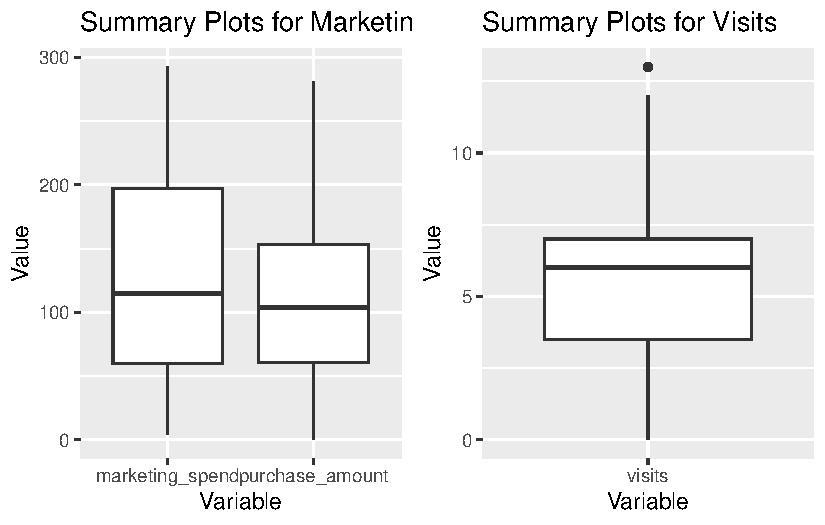
\includegraphics[keepaspectratio]{Assignment1_files/figure-pdf/summary-plots-1.pdf}}

\section{Results section}\label{results-section}

\begin{Shaded}
\begin{Highlighting}[]
\CommentTok{\# Summary plot}
\NormalTok{mar\_pur\_plot }\OtherTok{\textless{}{-}}\NormalTok{ data\_clean }\SpecialCharTok{|\textgreater{}}
  \FunctionTok{ggplot}\NormalTok{(}\FunctionTok{aes}\NormalTok{(}\AttributeTok{x =}\NormalTok{ marketing\_spend, }\AttributeTok{y =}\NormalTok{ purchase\_amount)) }\SpecialCharTok{+}
  \FunctionTok{geom\_point}\NormalTok{() }\SpecialCharTok{+}
  \FunctionTok{geom\_smooth}\NormalTok{(}\AttributeTok{method =} \StringTok{"lm"}\NormalTok{, }\AttributeTok{se =} \ConstantTok{FALSE}\NormalTok{, }\AttributeTok{color =} \StringTok{"blue"}\NormalTok{) }\SpecialCharTok{+}
  \FunctionTok{labs}\NormalTok{(}\AttributeTok{title =} \StringTok{"Marketing Spend vs Amount Purchases"}\NormalTok{,}
       \AttributeTok{x =} \StringTok{"Marketing Spend"}\NormalTok{,}
       \AttributeTok{y =} \StringTok{"Amount Purchases"}\NormalTok{) }

\NormalTok{mar\_vis\_plot }\OtherTok{\textless{}{-}}\NormalTok{ data\_clean }\SpecialCharTok{|\textgreater{}}
  \FunctionTok{ggplot}\NormalTok{(}\FunctionTok{aes}\NormalTok{(}\AttributeTok{x =}\NormalTok{ marketing\_spend, }\AttributeTok{y =}\NormalTok{ visits)) }\SpecialCharTok{+}
  \FunctionTok{geom\_point}\NormalTok{() }\SpecialCharTok{+}
  \FunctionTok{geom\_smooth}\NormalTok{(}\AttributeTok{method =} \StringTok{"lm"}\NormalTok{, }\AttributeTok{se =} \ConstantTok{FALSE}\NormalTok{, }\AttributeTok{color =} \StringTok{"blue"}\NormalTok{) }\SpecialCharTok{+}
  \FunctionTok{labs}\NormalTok{(}\AttributeTok{title =} \StringTok{"Marketing Spend vs Visits"}\NormalTok{,}
       \AttributeTok{x =} \StringTok{"Marketing Spend"}\NormalTok{,}
       \AttributeTok{y =} \StringTok{"Visits"}\NormalTok{) }

\NormalTok{pur\_vis\_plot }\OtherTok{\textless{}{-}}\NormalTok{ data\_clean }\SpecialCharTok{|\textgreater{}}
  \FunctionTok{ggplot}\NormalTok{(}\FunctionTok{aes}\NormalTok{(}\AttributeTok{x =}\NormalTok{ visits, }\AttributeTok{y =}\NormalTok{ purchase\_amount)) }\SpecialCharTok{+}
  \FunctionTok{geom\_point}\NormalTok{() }\SpecialCharTok{+}
  \FunctionTok{geom\_smooth}\NormalTok{(}\AttributeTok{method =} \StringTok{"lm"}\NormalTok{, }\AttributeTok{se =} \ConstantTok{FALSE}\NormalTok{, }\AttributeTok{color =} \StringTok{"blue"}\NormalTok{) }\SpecialCharTok{+}
  \FunctionTok{labs}\NormalTok{(}\AttributeTok{title =} \StringTok{"Visits vs Amount Purchases"}\NormalTok{,}
       \AttributeTok{x =} \StringTok{"Visits"}\NormalTok{,}
       \AttributeTok{y =} \StringTok{"Amount Purchases"}\NormalTok{)}

\NormalTok{mar\_pur\_plot}
\end{Highlighting}
\end{Shaded}

\begin{verbatim}
`geom_smooth()` using formula = 'y ~ x'
\end{verbatim}

\pandocbounded{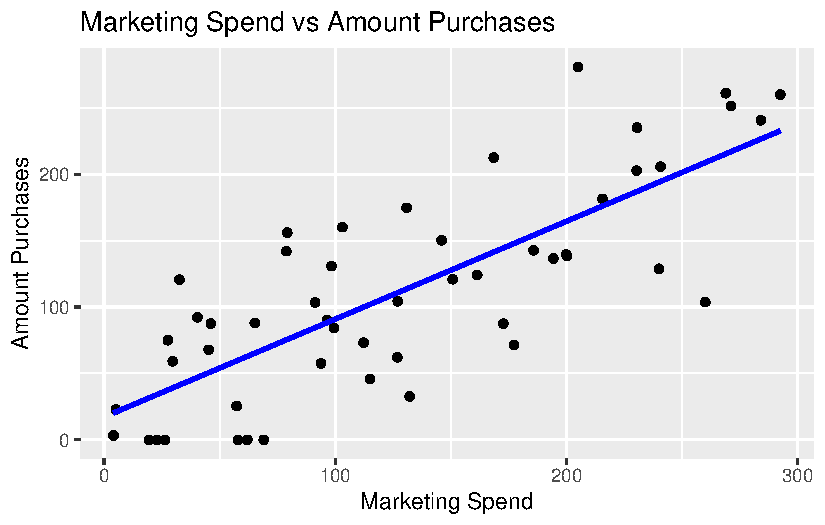
\includegraphics[keepaspectratio]{Assignment1_files/figure-pdf/relationship-plots-1.pdf}}

\begin{Shaded}
\begin{Highlighting}[]
\NormalTok{mar\_vis\_plot}
\end{Highlighting}
\end{Shaded}

\begin{verbatim}
`geom_smooth()` using formula = 'y ~ x'
\end{verbatim}

\pandocbounded{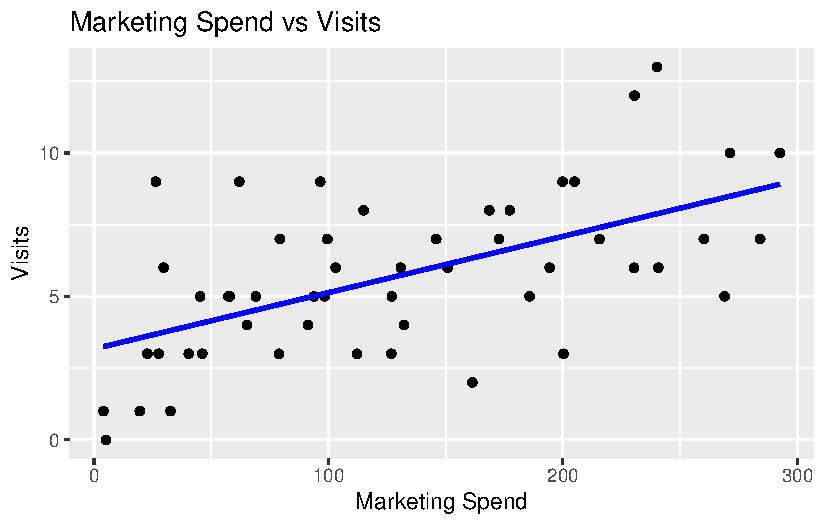
\includegraphics[keepaspectratio]{Assignment1_files/figure-pdf/relationship-plots-2.pdf}}

\begin{Shaded}
\begin{Highlighting}[]
\NormalTok{pur\_vis\_plot}
\end{Highlighting}
\end{Shaded}

\begin{verbatim}
`geom_smooth()` using formula = 'y ~ x'
\end{verbatim}

\pandocbounded{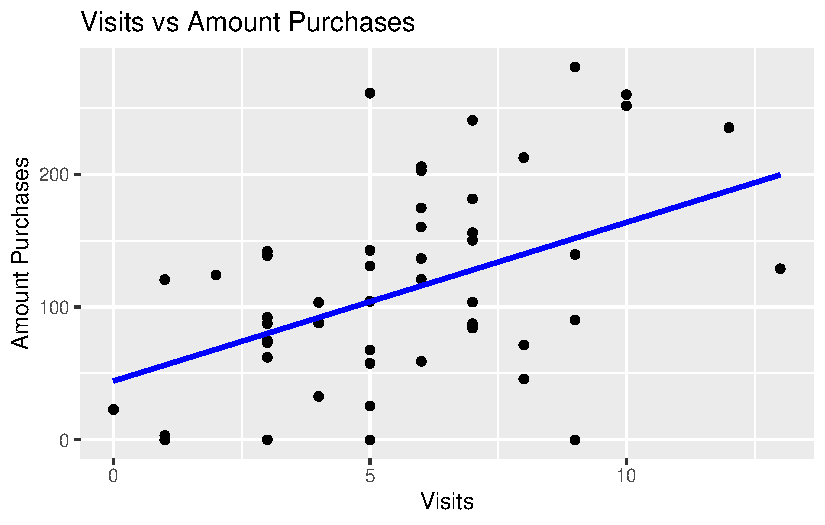
\includegraphics[keepaspectratio]{Assignment1_files/figure-pdf/relationship-plots-3.pdf}}

From the scatter plots, we can observe that there is a positive
relationship between marketing expenditure and the amount of purchases.
As marketing expenditure increases, we see an increase in purchase
amount, suggesting that higher marketing spend may lead to more customer
engagement and sales. However, there is just a weak relationship between
marketing expenditure and the number of visits. This indicates that
while marketing efforts may drive purchases, they do not strongly
increase the frequency of customer visits. And finally, there is a
positive relationship between the number of visits and the amount of
purchases. It is clear that customers who visit more frequently tend to
spend more, which suggests that encouraging repeat visits could be a key
strategy for increasing sales.

\section{Conclusion section}\label{conclusion-section}

In conclusion, our analysis of the dataset reveals that marketing
expenditure has a significant positive impact on the amount of
purchases, while its effect on the number of visits is relatively weak.
Additionally, there is a strong positive relationship between the number
of visits and the amount of purchases, indicating that customers who
visit more frequently tend to spend more. These findings suggest that
while investing in marketing can boost sales, strategies that encourage
repeat visits may be more effective in driving long-term customer
engagement and increasing purchase amounts.




\end{document}
